\section{Networks from freshly isolated samples} \label{s:p0}

% Introduce the work
This section presents the experiments on the second hypothesis made at the start of the chapter where a network representation of the gene expression form non-tumour will yield new \acrlong{mibc} subgroups. For this the gene expressions from the freshly isolated samples (P0 - \cref{s:lit:datasets_used}) was used to construct a co-expressed network following the pipeline in \cref{fig:N_I:network_pipeline}. The methods are almost identical with the previous section, where instead of tumour's gene expression the P0's RNAseq data is used. The mutation burden used for the edges' weight modifier is still from TCGA. 

% Implication on the network pipeline
% Limitation of using this method as only a gene selection method
Having a non-tumour network  means that the \gls{MODCON} (ModCon) selects the genes that are most representative of the communities in the P0 samples. These genes are then used to compute the Module Evaluation Value (MEV) score using the gene expression from TCGA. In short, this is a method to select the genes most representative for the freshly isolated samples, being the closest molecular depiction of the bladder tissue, and how their expression in the tumours dataset inform the MIBC subtyping.

% Caution on the small datasets
P0 samples are an invaluable dataset, as they are the closest representation of healthy bladder tissue and hold significant potential for uncovering new biological insights. However, the small number of P0 samples—only 23 may limit the statistical power to detect communities with specific biological functions. In addition, the MIBC cohort contains de-differentiated and trans-differentiated samples, which may be poorer represented by the P0 datasets.


% Why choosing the high number of TF
The minimum degree for TF was pseudo-empirically chosen by generating several networks with TF degrees ranging from 10 to 100 (in increments of 25) and visualising them in Gephi. It was observed that networks with a higher number of edges were very nested yielding lower scores. Initially, it was assumed that the Leiden algorithm would not be heavily influenced by allowing TF (approximately 325 of 4,000 genes) more links. To put this in perspective, the Spearman correlation matrix is 4,000x4,000, and each gene has 3,999 correlations. Thus, keeping 100 edges per TF is not excessive.

% However, the experiments in this section and the work in \cref{s:ap:sel_prun} will show that allowing such a large number of TF has a big impact on the number of communities.

% In PGCNA \citet{Care2019-ij} select in each community the top 25 genes with the highest ModCon score. This was the initial value used in the P0 experiments too but many genes are missed, where communities in the healthy were not expressed in tumours. Thus, it was increased to 100. On top of that, when computing the MEV scores using the tumour gene expression it was used only the top 4000 most varied genes in the MIBC. This aggressive strategy for MEV was to include the genes that are both the most varied in the tumour and P0 samples, the results for this are covered in \cref{s:N_I:gene_rep}.

In this section the top 4K most-relative varied genes (median/std) from P0 are used to construct the network, the same weight modifiers (Reward and Penalised see Figure \ref{fig:N_I:modifiers}) are employed and 50 edges for the Transcription Factors. For the standard genes 3 edges are kept while for \acrlong{tf} 50. The top 100 genes are selected with ModCon and for MEVs the top 4000 most varied genes are used.

% Desribe the network
\subsection{Network description} \label{s:N_I:p0_tum_description}

% Introduce the metrics
The same five network metrics in the previous sections are used for the P0-derived graph: degree, PageRank, closeness, betweenness, and IVI, introduced in \cref{s:lit:net_metrics}. These metrics provide an overview of the network properties, including how well the nodes are connected, their shortest paths, and their overall importance (IVI).


\begin{figure}[!b]    
    \centering
    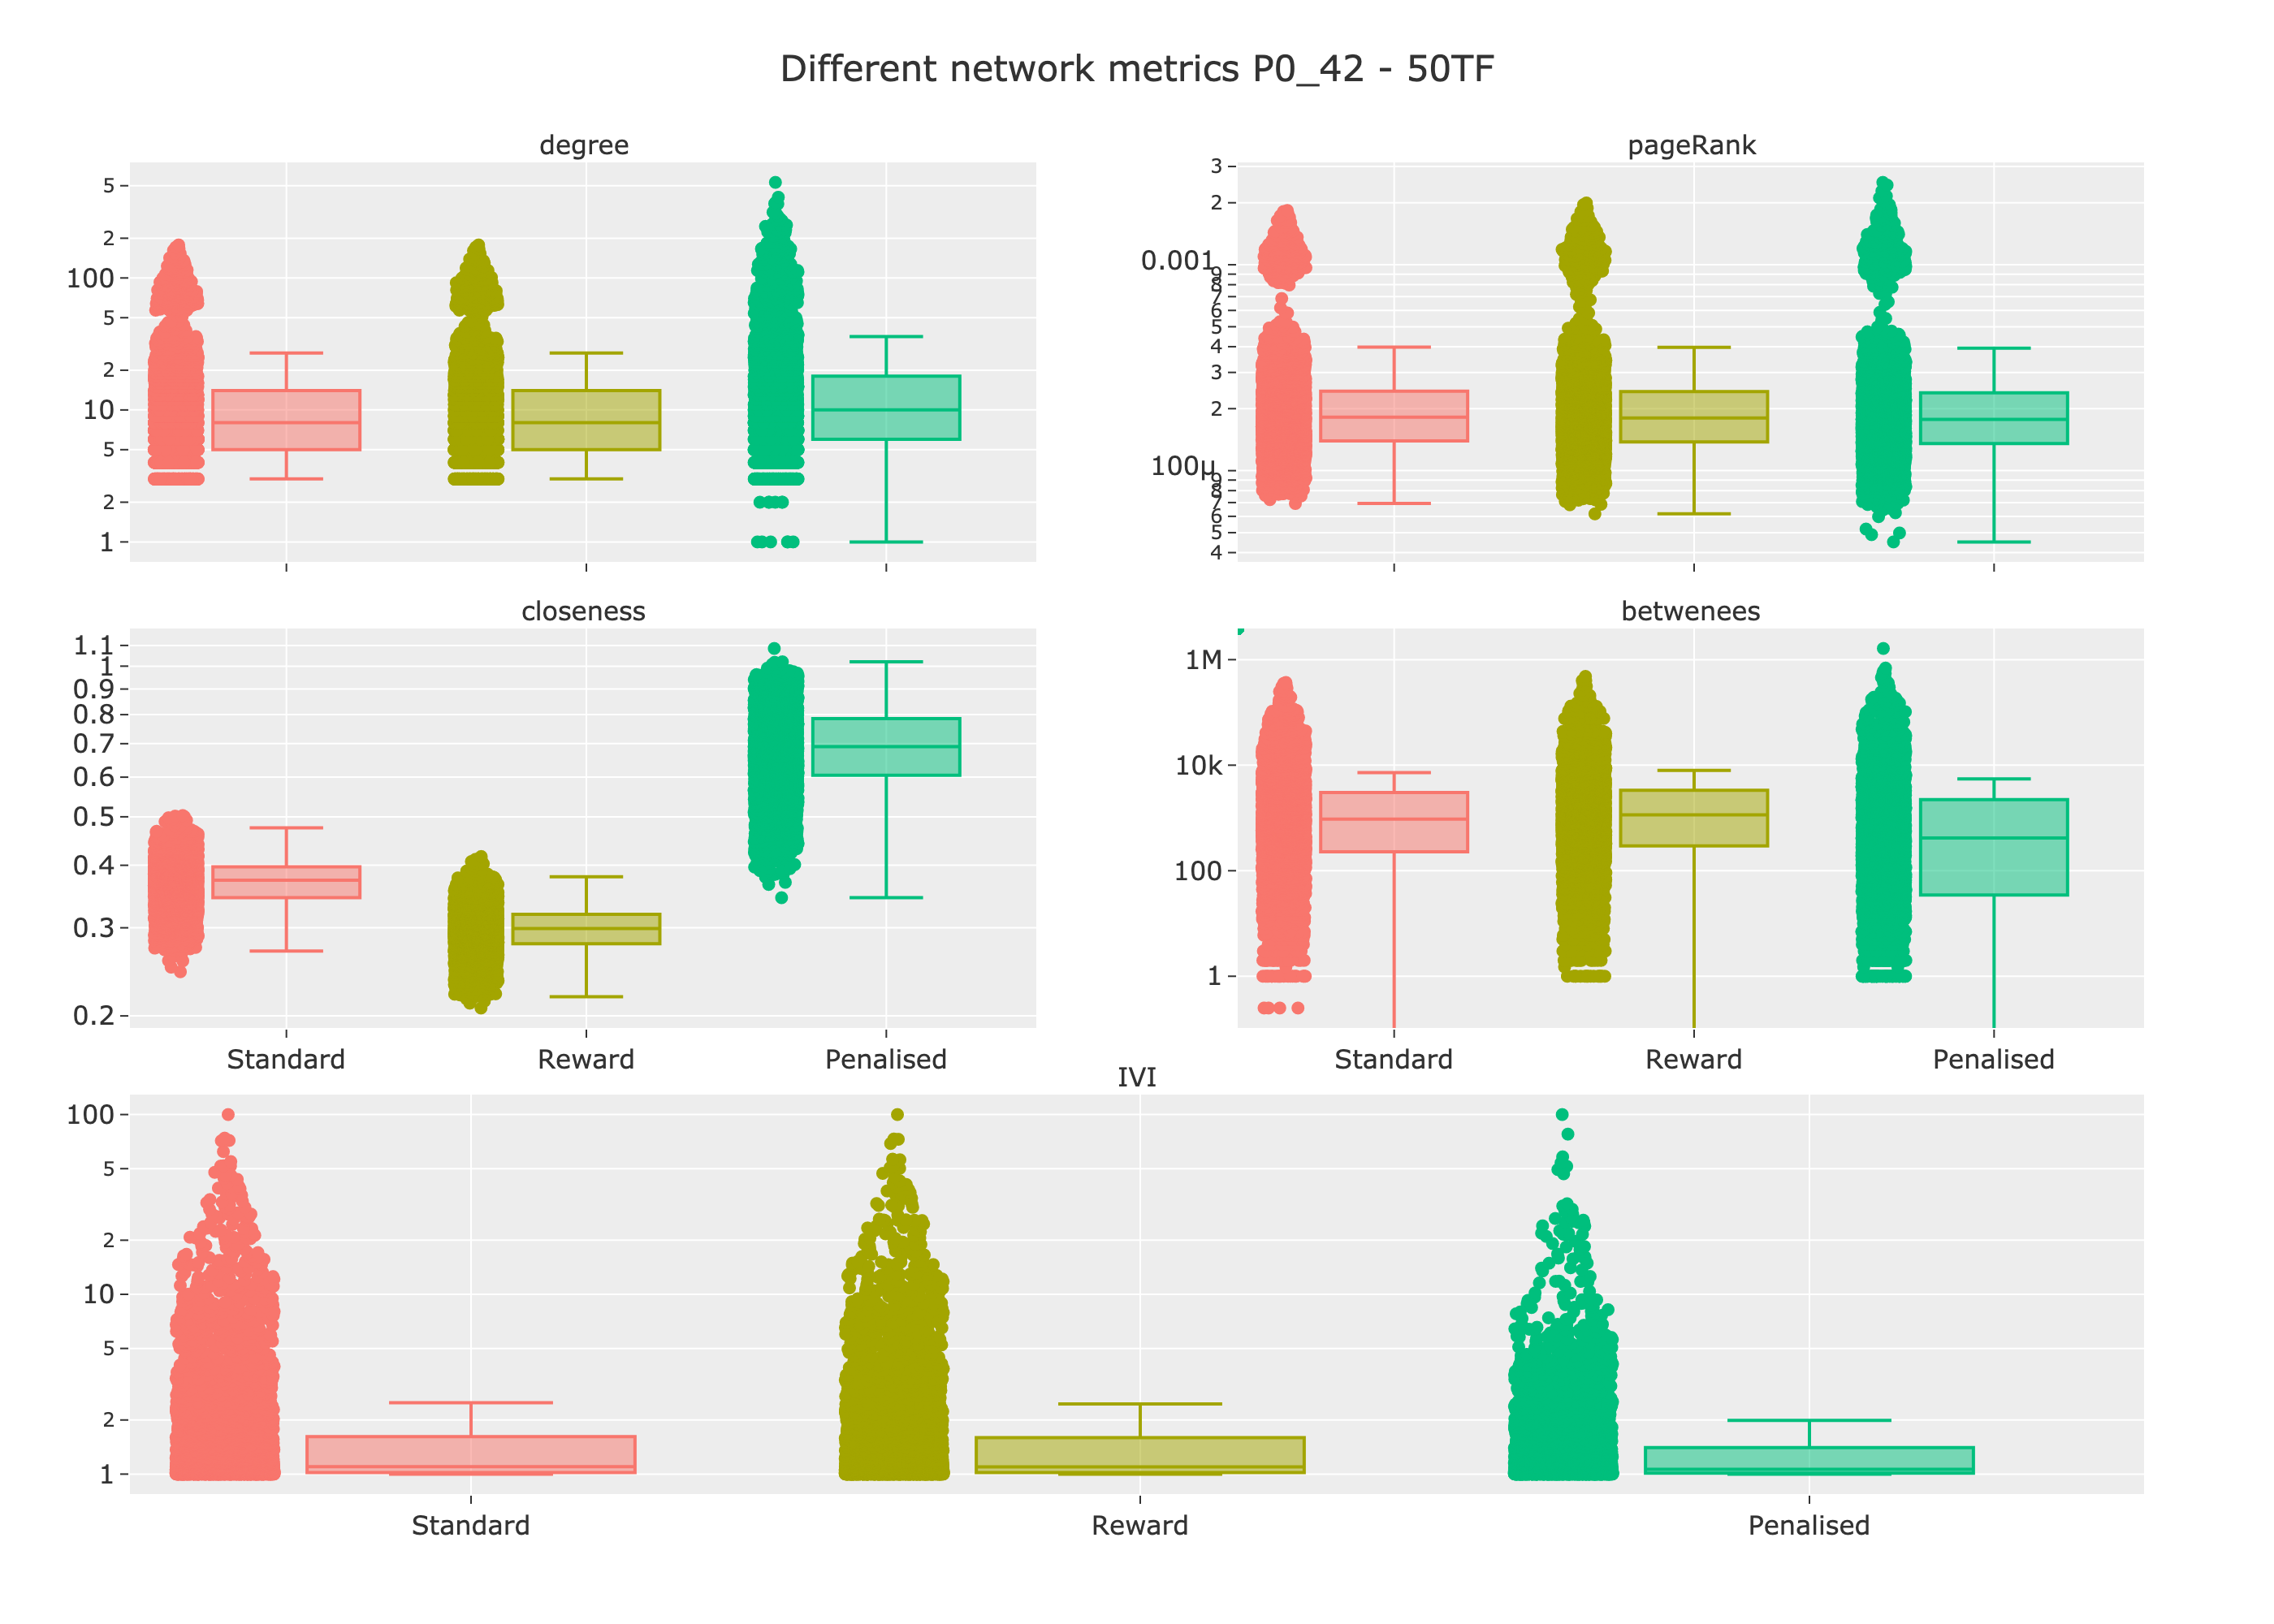
\includegraphics[width=1.0\textwidth,keepaspectratio]{Sections/Network_I/Resources/P0/P0_NetworkMetricsComp_50TF_2.png}
     \caption[P0: centrality network metrics]{Network metrics for the P0 networks formed from 4K genes, 3 connections per standard gene and 6 for TF with the different weight modifiers; standard (red), reward (mustard) and penalised (green). The y-axis represent is in log scale of the metric. Higher the degree and pageRank values more important the node is to the network, smaller values of closeness metric indicates that the vertices are closer together, while higher values of betweenness means that a node serves as a key bridge between other nodes. Higher values of \acrlong{ivi} indicates the node has a large influence both locally and globally to the network. Overall, the P0 networks have nodes with a larger number of connections and are closer together compared to the tumour networks. The nodes in the reward network become closer together compared with the standard graph and the opposite effect is seen in the penalised network. }
    \label{fig:N_I:net_metrics_p0}
\end{figure}


% Cone-shaped number of edges - a subset of genes closer together
In the standard and reward networks, there is a subset of more connected nodes, with a noticeable difference from the rest of the nodes. This is illustrated by the cone-shaped distribution of the degree metrics, which comprises more than 200 nodes in each network, each having more than 50 connections; see \cref{fig:N_I:net_metrics_p0}. The aspect, which is less visible in the penalised network, has a significantly different degree distribution from the standard and reward graphs (\acrshort{kw}: 103.806,p-value: $2.870e^{-23}$).

The PageRank metric exhibits a similar trend, where a subset of vertices is noticeably more critical in the network than the others; this pattern is present across all three networks. However, the distribution of the score across the three networks is marginally significant (\acrshort{kw}: 5.829,p-value: 0.0542). The similar median values across the two centrality metrics can be explained by the fact that the penalised weight modifier does not remove connections but merely reduces their weights to a small value. Another effect of reducing the weight is that the penalised network has a higher spread in the degree, reaching nodes with almost 500 connections. In contrast, the maximum degree for the standard and reward networks is about half of this.

\begin{table}[!b]
  \centering
  \small
  \begin{tabularx}{\textwidth}{>{\hsize=.25\hsize}X|>{\hsize=.35\hsize}X|>{\hsize=.35\hsize}X|>{\hsize=.35\hsize}X}
    \toprule
    \textbf{Metric} & \textbf{Standard vs Reward} & \textbf{Standard vs Penalised} & \textbf{Reward vs Penalised} \\
    \midrule
    \textbf{Betweenness} & 7606550.0; $1.39e^{-4}$ & 9529730.5; $3.11e^{-50}$ & 9862132.5; $2.03e^{-73}$ \\
    \midrule
    \textbf{Closeness} & 14796488.0; 0.0 & 47620.0; 0.0 & 481.0; 0.0 \\
    \midrule
    \textbf{Degree} & 8025726.5; 0.803 & 7095557.5; $3.25e^{-18}$ & 7071269.0; $3.96e^{-19}$ \\
    \midrule
    \textbf{PageRank} & 8092890.0; 0.368 & 8239617.0; 0.0164 & 8144402.0; 0.140 \\
    \midrule
    \textbf{IVI} & 8076343.0; 0.460 & 8823832.0; $7.65e^{-16}$ & 8749049.0; $2.21e^{-13}$ \\
    \bottomrule
  \end{tabularx}
  \caption[P0: Network metrics significance]{P0 networks metrics comparison of Betweenness, Closeness, Degree, PageRank, and IVI metrics across standard, reward, and penalised networks. The first value is represented by the result from the \acrlong{mw} while the second the p-value.}
  \label{tab:N_I:p0_net_metrics}
\end{table}

% Closeness
A significant difference between the penalised network and the other two graphs is that the former has nodes that are more spread apart (\acrshort{kw}: 9885.138,p-value: 0), as shown by the closeness metric in \cref{fig:N_I:net_metrics_p0}. The betweenness distributions are significantly different across the three networks (\acrshort{kw}: 376.559,p-value: $1.702e^{-82}$), indicating that the networks have different connecting nodes. The IVI distribution of the IVI scores was significantly different for the penalised network (\acrshort{kw}: 79.529,p-value: $5.373^{-18}$), suggesting that different nodes have local and global importance in the standard and reward networks.

The P0 penalised network is significantly different from the other two networks (see \cref{tab:N_I:p0_net_metrics}), suggesting that reducing the weights to values close to 0 for highly mutated genes has a greater impact on the network than rewarding them by doubling their values. This might be explained that the edges are almost pruned when the penalised edge weight modifiers is applied.

% Comparing the scales


\paragraph*{Comparing with the tumour networks}

There are significant differences (see \cref{tab:N_I:tum_p0_comp}) between the graphs derived from the P0 dataset compared to those generated from the tumour dataset; see \cref{fig:N_I:net_metrics_tum}. The P0 networks appear to be more densely connected, with nodes that are closer together and exhibit greater variance in the degree and closeness metrics. The nodes in the P0 network have a median degree of around 10, while those in the tumour networks have a median degree of around 4. The distribution of connections in the P0 network is also skewed to the right, with an upper fence greater than 10, whereas in the tumour networks, the upper fence is less than 10. This is also reflected in other metrics, such as closeness, where the vertices in the P0 network are closer than those in the tumour graphs.


Overall, the P0 networks have nodes with a larger number of connections and are closer together compared to the tumour networks. A subset of nodes with a larger degree means that there are some genes that are more correlated with other genes compared to the normal, as it was found in \cref{s:N_II:high_conn}. The three graphs in this section share a subset of highly connected genes, as seen in the PageRank and Degree plots from \cref{fig:N_I:net_metrics_p0}. This can be explained by the TF genes, which allowed at least 50 connections per node compared to 3 for the standard genes. 

\begin{table}[!htb]
  \centering
  \small
  \begin{tabularx}{\textwidth}{>{\hsize=.23\hsize}X|>{\hsize=.33\hsize}X|>{\hsize=.35\hsize}X|>{\hsize=.36\hsize}X}
    \toprule
    \textbf{Metric} & \textbf{Standard (s)} & \textbf{Reward (s)} & \textbf{Penalised (s)} \\
    \midrule
    \textbf{Betweenness} & 4070919.5; 0.0 & 4387136.5; $4.51e^{-268}$ & 3929074.5; 0.0 \\
    \midrule
    \textbf{Closeness} & 14508764.0; 0.0 & 14236214.0; 0.0 & 15237386.0; 0.0 \\
    \midrule
    \textbf{Degree} & 12007459.0; 0.0 & 12039960.0; 0.0 & 12302430.5; 0.0 \\
    \midrule
    \textbf{PageRank} & 7153799.0; $2.55e^{-16}$ & 7155816.0; $3.00e^{-16}$ & 6482391.0;  $2.50e^{-41}$ \\
    \midrule
    \textbf{IVI} & 7399455.0; $6.09e^{-09}$ & 7428084.0; $3.07e^{-08}$ & 5540028.5; $3.13e^{-114}$ \\
    \bottomrule
  \end{tabularx}
  \caption[Tum vs P0 network metrics significance]{Results of \gls{mw} between the betweenness, closeness, degree, PageRank, and IVI metrics of the P0 and tumour-derived networks. The first value is the result from the \acrshort{mw} test while the second is the p-value. Each network derived from the tumour dataset is compared with its equivalent from the non-tumour. The results show there is significant difference in the network metrics.}  \label{tab:N_I:tum_p0_comp}
\end{table}


% Network comparison
\subsection{Network comparison}

% Introducing
\Cref{fig:N_I:p0_sky_leiden} represents an overview of the MIBC groups derived from the thee non-tumour networks, results which are put in the context of the other classifications: consensus \citep{Kamoun2020-tj}, TCGA sub-grouping \citep{Robertson2017-mg} and the previous work on clustering analysis (see \cref{s:clustering_analysis}). K-means with K=5 was applied across all three networks and for a more in-depth clustering analysis see \cref{s:ap:P0_cs_analysis} from Appendix.

% Present the results
There is no significant difference (\acrshort{kw}: 0.979, p-value: 0.61) between the range of communities found by Leiden in all three networks, with between 9 and 11 communities found in each case. This is less than half the number of blocks in the networks created from the tumour dataset (\cref{fig:N_I:tum_leiden_modifiers}), which also exhibited greater variability. There are significant differences between the community metrics for the networks derived from tumour and non-tumour datasets, see \cref{tab:N_I:modularity_module_num_comp}. The difference might be explained by the fact that malignant tumours exhibit multiple and distinct dysregulations of normal cellular processes, whereas, in the benign samples from P0, these processes are less disrupted. In addition, the tumour contains cell types that are not present in the P0 dataset.


\begin{figure}[!b]    
    \centering
    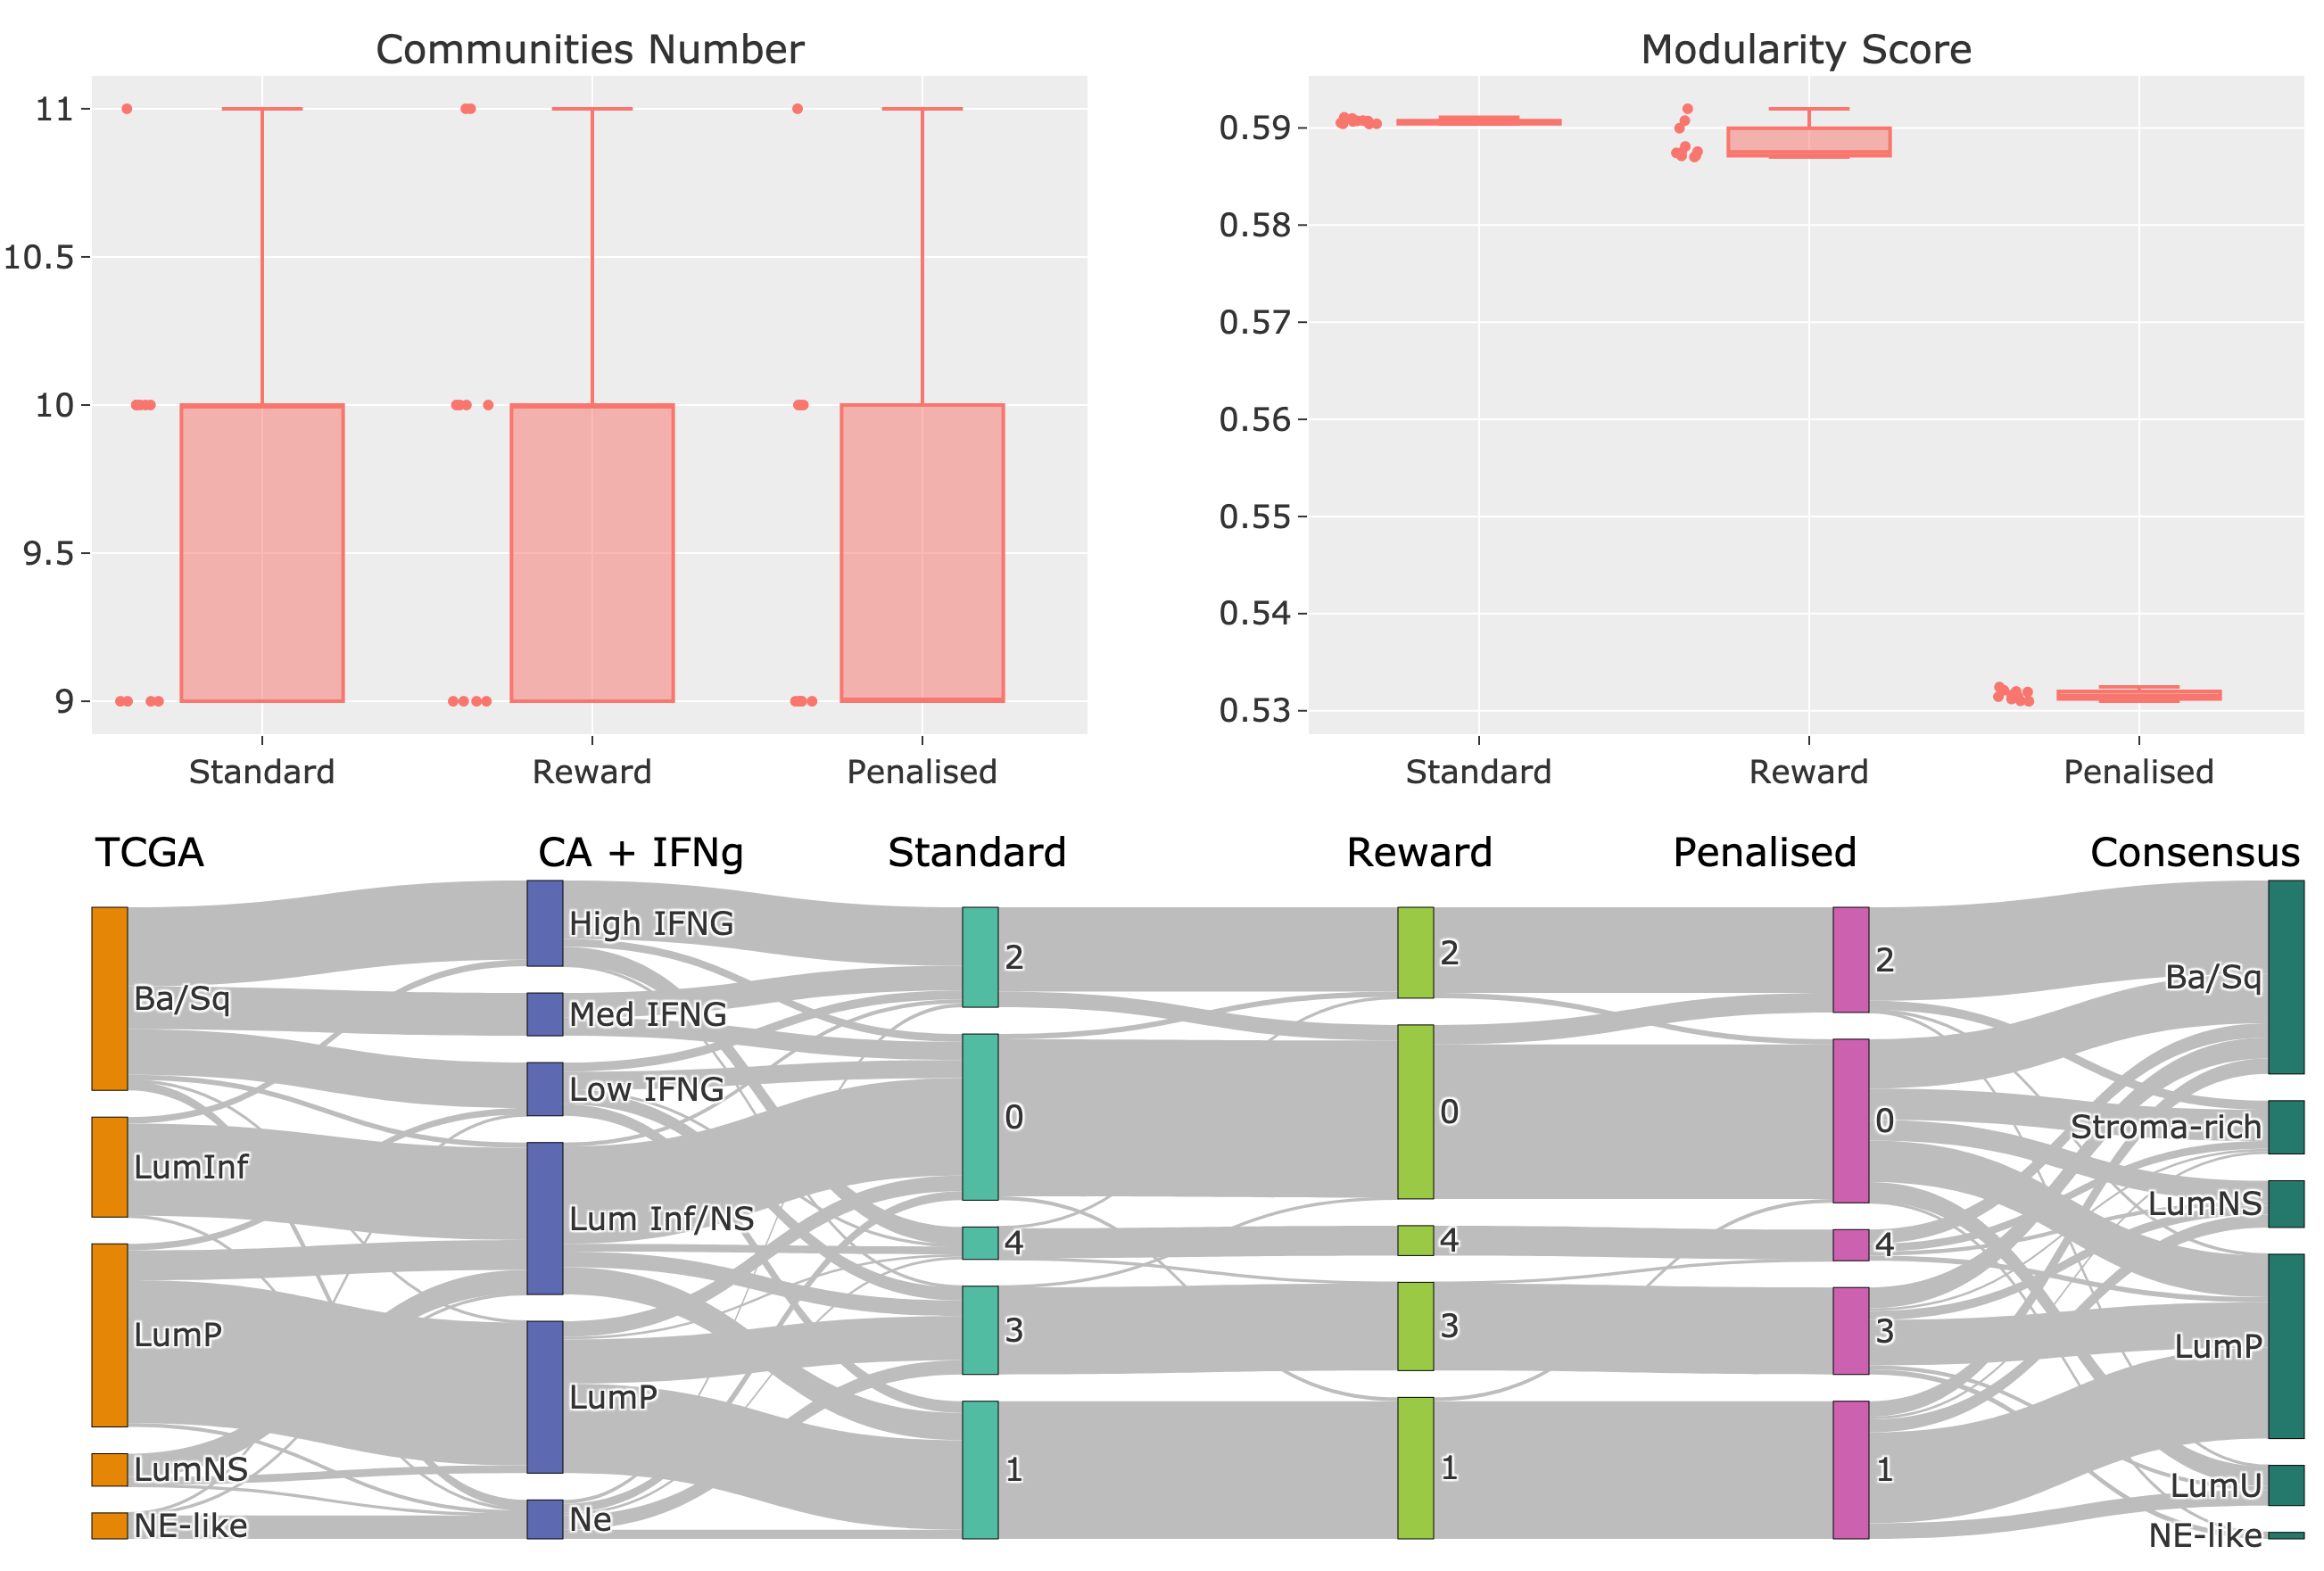
\includegraphics[width=1.0\textwidth,keepaspectratio]{Sections/Network_I/Resources/P0/Ldn_Sky_TF_50_RawKMeans_K5_v3.png}
    \caption[P0: Leiden metrics]{Overview of the MIBC groups found using the expression from the P0 dataset. On the top are displayed the community size and Modularity Score. The two metrics used to asses effects of the weight modifiers (standard, reward and penalise) to the Leiden algorithm. At the bottom the Sankey plot displays comparison between the MIBC subtyping derived from the different standard classifiers (TCGA \citep{Robertson2017-mg} and consensus \citep{Kamoun2020-tj}), the previous developed subgroups with the cluster analysis \cref{s:clustering_analysis} and the three different networks. The figures show that there are less communities found compared with the tumour networks and there is less variance on the MIBC subtyping across the P0 derived networks. }
    \label{fig:N_I:p0_sky_leiden}
\end{figure}

% Talk about the variance in Modularity score
The small variance in the Modularity score, as shown in the figure on the right, suggests that the communities are fairly stable, with the penalised network performing lower by 0.04. Compared to the tumour networks, the P0-derived graphs exhibit a significantly lower performance by 0.02 (\acrshort{kw}: 22.165,p-value: $1.537e^{-05}$). This indicates that the communities in the non-tumour networks are not as well separated as those in the tumour-derived networks. This observation aligns with the network metrics discussed in \cref{s:N_I:tum_describe}.

It is striking the lack of change across the subtypes derived from the P0 networks as seen in the Sankey plot from the bottom of \cref{fig:N_I:p0_sky_leiden}. Cluster \textbf{2} holds most of the High INFG (from CA+INFG), group \textbf{0} is a mixed of the other Basal groups combined with the luminal infiltrated and \textbf{4} is a small subset of High IFNG. The luminal groups are combined in two clusters \textbf{3} and \textbf{1}.


\begin{table}[!htb]
  \centering
  \small
  \begin{tabularx}{\textwidth}{>{\hsize=.4\hsize}X|>{\hsize=.3\hsize}X|>{\hsize=.3\hsize}X|>{\hsize=.3\hsize}X}
    \toprule
    \textbf{Metric} & \textbf{Standard} & \textbf{Reward} & \textbf{Penalised} \\
    \midrule
    \textbf{Modularity Score} & 0.0; $1.83e^{-04}$ & 0.0; $1.83e^{-04}$ & 0.0; $1.83e^{-04}$ \\
    \midrule
    \textbf{Module Number} & 0.0; $1.43e^{-04}$ & 0.0; $1.29e^{-04}$ & 0.0; $1.17e^{-04}$ \\
    \bottomrule
  \end{tabularx}
  \caption[Tum vs P0: Modularity and Module Number Comparison]{Results of \gls{mw} for the modularity score and module number between the P0 and tumour-derived networks. Each network derived from the tumour dataset is compared with its equivalent from the non-tumour: Standard derived from tumour vs Standard build from non-tumour. The results show there is significant difference in the community detection metrics.}
  \label{tab:N_I:modularity_module_num_comp}
\end{table}


Overall, the comparison between classifications shows that the network approaches exhibit different subtypes from the other traditional methods.  Several samples change group membership in the three different networks, but there are no large changes. This contrast with the MIBC subgroups found in the work on tumour derived networks where there the weight modifiers had a larger impact on the disease stratification. In addition,  three are fewer communities found and less clearly defined compared with blocks found in the tumour derived networks. 


% From the Sankey plot it can be seen that the High IFNG group (CA+IFNg) is contained across the 3 networks in cluster \textbf{2}. Groups \textbf{2} in Standard and Penalised are similar and formed mostly from Ba/Sq groups while cluster \textbf{1} (Reward) has additional samples from LumInf/NS\footnote{Would this mean that by increasing the weight values more samples are added to the group? While pruning edges removes some of the noise?}. The cluster \textbf{0} from the Standard network resembles to the LumInf/NS group from the CA+IFNG classification, being a mixed of samples. Group \textbf{ 0} (Reward and Penalised) and \textbf{1} (Standard) contains samples which previously were considered Luminal samples. Lastly, cluster \textbf{4} contains a consistent number of samples which previously classified as High IFNG.

% Community analysis
\subsection{Community analysis} \label{s:N_I:com_analysis}

Previous sections showed that the weight modifiers have an impact on the P0 derived graphs but had little impact on the MIBC stratification. This is in contrast with what was observed in the analysis of the tumour networks, see \cref{s:N_I:tum}. To further understand the differences, the next step is to analyse the changes in communities when a modifier is applied. There are a few questions to answer 1) How do the communities change? 2) Is there a shift in the overall mutation burden of a block? 3) What is the gene expression difference between the groups? 

% Introduce the analysis of the communities with the mutations
To facilitate analysis, and guided by the Modularity Score, the standard and reward networks with the highest Modularity Score were selected for community comparison which are shown in \cref{fig:N_I:p0_chg_sankey}. The blocks of genes from the two graphs are aligned with the method described in \cref{s:ap:align_coms} from Appendix.

% gene migration
\subsubsection*{Changes in communities}

% Comment on the Sankey
% Not that many changes
The largest change in communities is represented by the lack of block 10 in the reward network, otherwise the communities are remarkably similar; see  Sankey plot \cref{fig:N_I:p0_chg_sankey} Again indicating that the weight modifiers are not powerful enough to have a stronger influence on the Leiden community detection algorithm. 

% Link it with the mutations
As it was mentioned earlier if there is any membership change across the blocks of nodes it is influenced by the mutated genes. For each group it can be usually notice that the there is a large number of mutated genes from the same community. In the reward network community 1 has a large number of mutations which was also presented the standard network (red dotted) and it receives a few more mutated genes from community 2 (blue); shown in \cref{fig:N_I:p0_chg_mut}. Community 4 from the modifier graph retain most of the mutated genes from the standard (community 5 - orange) with some additional genes from community 6 (purple). Blocks 8 and 9 have a few mutated genes which can be in part explained by their small group size. 

Overall, the analysis suggests that the reward modifier triggers gene community migrations between the two graphs which further proves that the data integration does happen in the modified network. However, as it was shown by the Sankey there are no large changes across the blocks which may explain why the MIBC groups do not change with the different networks.

% Comment on the sankey and the mutations
\begin{figure}[!htb]
    \centering
    \begin{subfigure}[!t]{1.0\textwidth}
        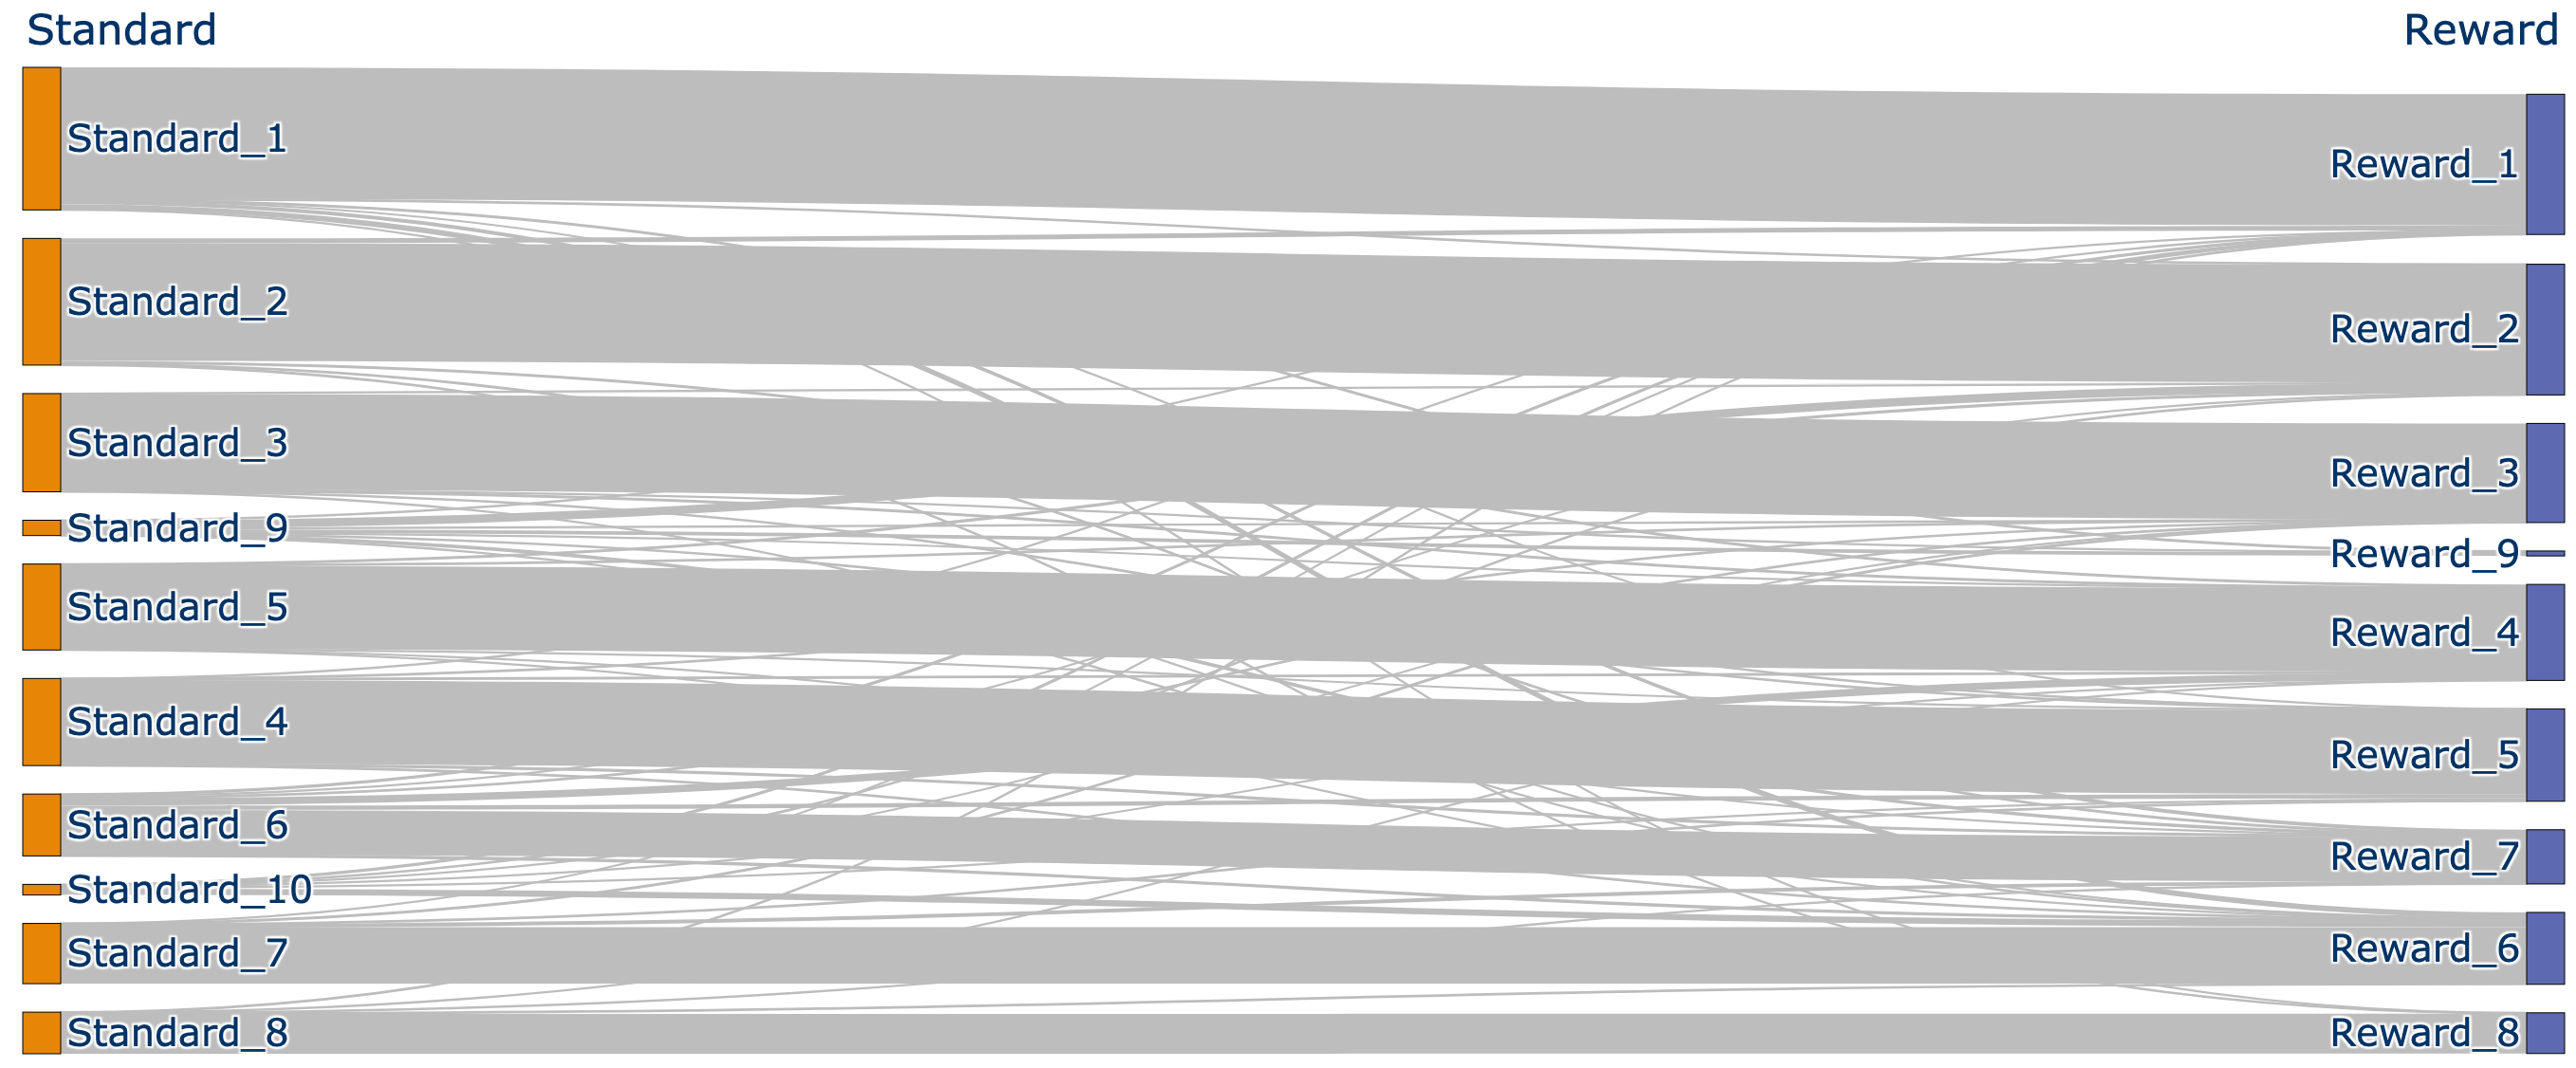
\includegraphics[width=\textwidth,keepaspectratio]{Sections/Network_I/Resources/P0/Comms/Sky_Comm_Comp_4K_v3.png}
        \caption{Gene changes across the communities in Standard and Reward network}
        \label{fig:N_I:p0_chg_sankey}
    \end{subfigure}
    \begin{subfigure}[!t]{1.0\textwidth}
        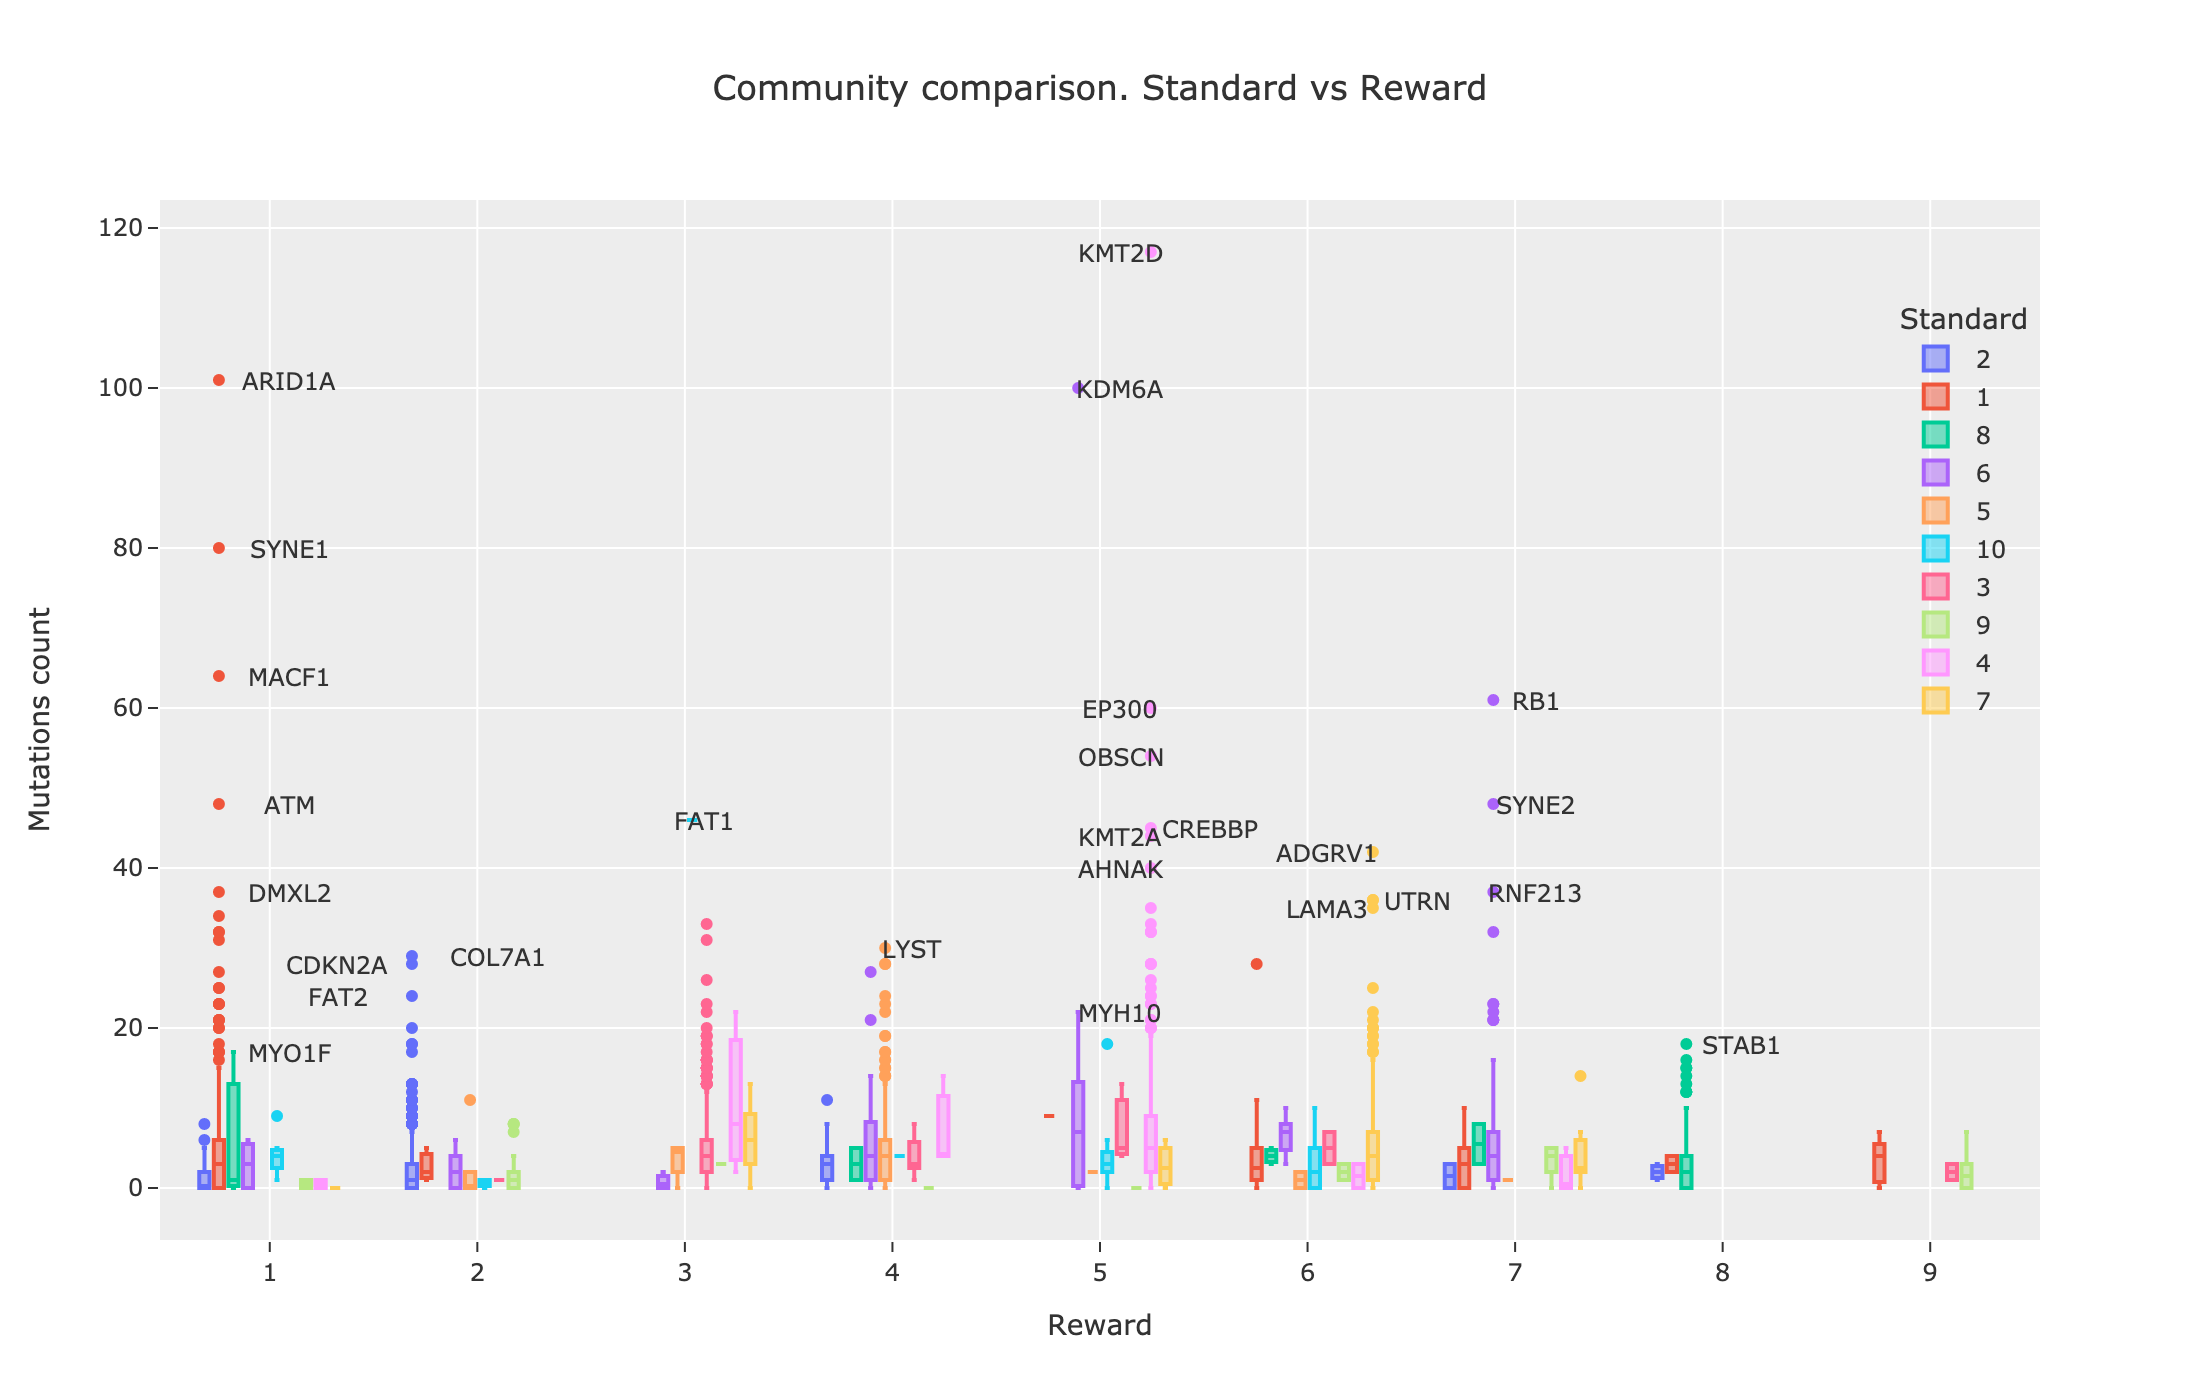
\includegraphics[width=\textwidth,keepaspectratio]{Sections/Network_I/Resources/P0/Comms/Mut_Comm_Comp_4K_v3.png}
        \caption{Mutation burden across communities}
        \label{fig:N_I:p0_chg_mut}
    \end{subfigure}
    \caption[Gene migrations between communities]{Gene communities changes (A) and their corresponding mutation burden (B). The X-axis in B) represent the communities in which the genes are in the reward network after the modifier was applied (or right-hand side in the Sankey plot) and the colours represent the communities in the standard network (left-hand side in the Sankey plot). The first figure indicates that the weight modifiers work by causing gene membership changes while the second plot show that the communities retain most of the genes mutated suggesting that the weight modifier are not powerful enough to cause larger changes across the blocks. }
    \label{fig:N_I:p0_comm_chgs_1}
\end{figure}



% Expression across communities
\subsubsection*{High mutation burden}

% Why are we doing this
The strip plot from \Cref{fig:N_I:p0_chg_mut} is a suitable figure to show that most communities from standard network retain their mutated genes after the weight modifier is applied, but it is qualified too check if the reward modifier affects the genes with the higher mutation burden. Are the genes with the highest mutation count grouped together?

% Highly mutated genes are changing the communities
\Cref{fig:N_I:p0_mut_burden} shows the evolution of the mutation burden across communities. In the standard, communities 1, 2, 3, 4 and 5 have the highest number of genes mutated and it can be noticed that all have the same trend a sharp decline after mutation burden $>1$; community 4 having the highest number of highly mutated genes. Similar trends can be noticed in the reward network but communities 2,3,4 have a similar slope. In addition, community 9 has just a few mutation with low burden, while 6 and 7 are better separated in the reward. This changes suggests that the highly mutated genes are the ones changing communities.

% Comment on gene expression
With few gene changes across the communities in the two graphs, there is also little change in the median gene expression between the standard and reward networks. This is shown in the box plots from \cref{fig:ap:p0_ge_chgs} in Appendix \cref{s:ap:ge_p0_com}. Communities 1 and two are almost unchanged in the reward network while in the others the spread of the median expression is affected. The largest difference is in community 9 and 3.  

% Conclusion 1 - Weight modifiers work
Overall, the community analysis shows that the reward modifier works, there are changes between communities and this is given by the mutated genes, especially the ones with a high burden. Nevertheless, the results indicate that a new weight modifier with a gradual, proportional change with the mutation burden will have a larger impact in the networks; this is introduced in \cref{s:N_II}.

\begin{figure}[!htb]
    \centering
    \begin{subfigure}[b]{1.0\textwidth}
        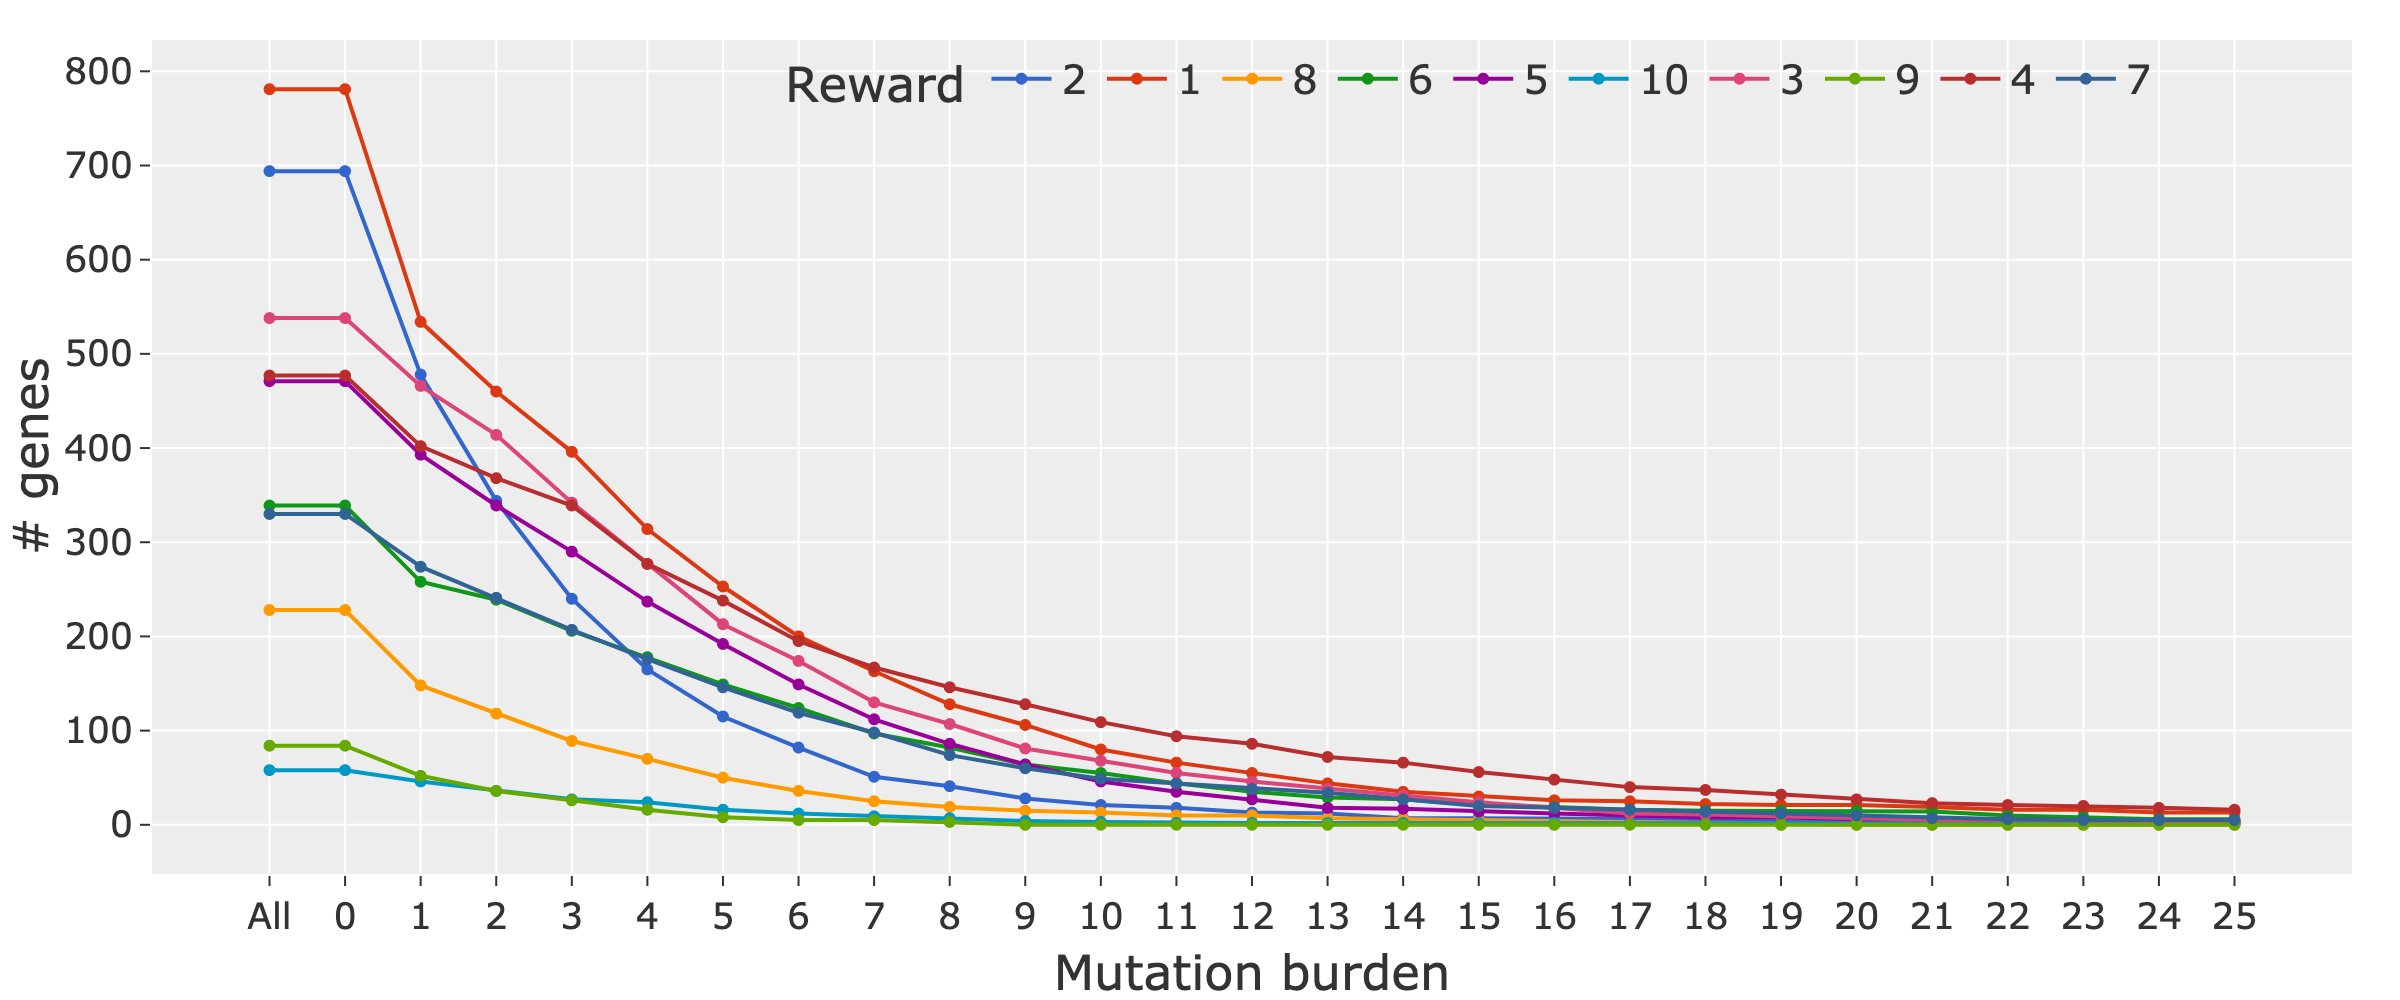
\includegraphics[width=\textwidth,keepaspectratio]{Sections/Network_I/Resources/P0/Comms/Mut_evo_Std_4k_v3.png}
        \label{fig:N_I:p0_std_mut_burden}
        \caption{Standard}
    \end{subfigure}
    \begin{subfigure}[b]{1.0\textwidth}
        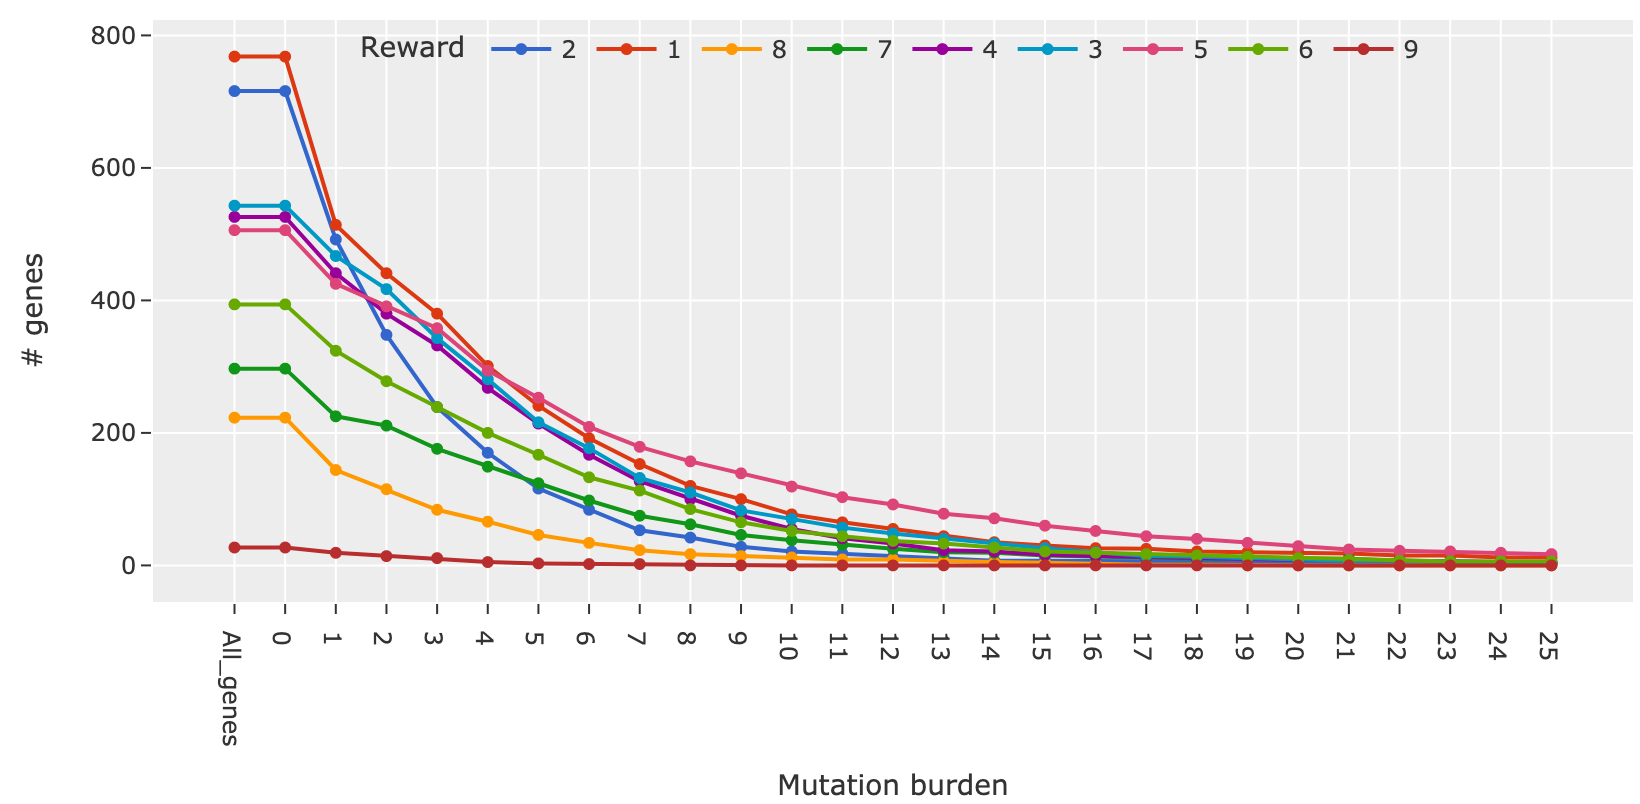
\includegraphics[width=\textwidth,keepaspectratio]{Sections/Network_I/Resources/P0/Comms/Mut_evo_Rwd_4k_v3.png}
        \caption{Reward}
        \label{fig:N_I:p0_rwd_mut_burden}
    \end{subfigure}
    \caption[Mutation burden per communities]{These two plot show how many genes are included in each community as the mutation burden increases.}
    \label{fig:N_I:p0_mut_burden}
\end{figure}


\subsection{Gene representation} \label{s:N_I:gene_rep}

It is worth remembering that the co-expressed networks are constructed from the gene expression data of the P0 samples and that only the genes selected with ModCon are used to stratify the MIBC. Differences in gene expression between the two datasets are expected; some genes may be expressed in the freshly isolated samples but not in the tumour, and vice versa. Additionally, the genes used to compute the MEV score were limited to the top 4000 most varied genes, ensuring variability across both datasets. It is therefore important to understand the implications of these decisions and assess how well the genes selected through ModCon and MEV are represented in the tumour dataset.

% Introduce the bar plot
To study these differences, only the reward network is presented in this section, while the standard network is covered in the Appendix (\cref{s:ap:p0_gene_rep_std}). The top 100 genes from each community were selected using the ModCon score, and their representation is shown in both the 4000 most varied genes (\cref{fig:N_I:p0_mev_sel_rep}) and all the expressed genes (\cref{fig:N_I:p0_mev_all_rep}) in the tumour dataset.

% Conclusion - Poor representation
From the two figures, it is evident that using only the most varied genes results in a significant number of missing genes, and the same pattern is observed for the standard network in \cref{fig:ap:std_p0_mev_rep}. This poor representation might explain the lack of differences between the MIBC subtypes derived from the reward/penalised networks, as seen in \cref{fig:N_I:p0_sky_leiden}.

Nevertheless, even when all expressed genes are considered, some genes are still missing. One possible explanation is that a larger dataset is needed to form the network, including a molecular representation of the basal groups, such as undifferentiated samples from non-tumours. Another reason could be that the gene filtering used in \cref{s:cs:pre-processing} is too aggressive, discarding too many genes and leading to a poor match between tumour and non-tumour expressed genes.


\begin{figure}[!htb]
    \centering
    \begin{subfigure}[b]{1.0\textwidth}
        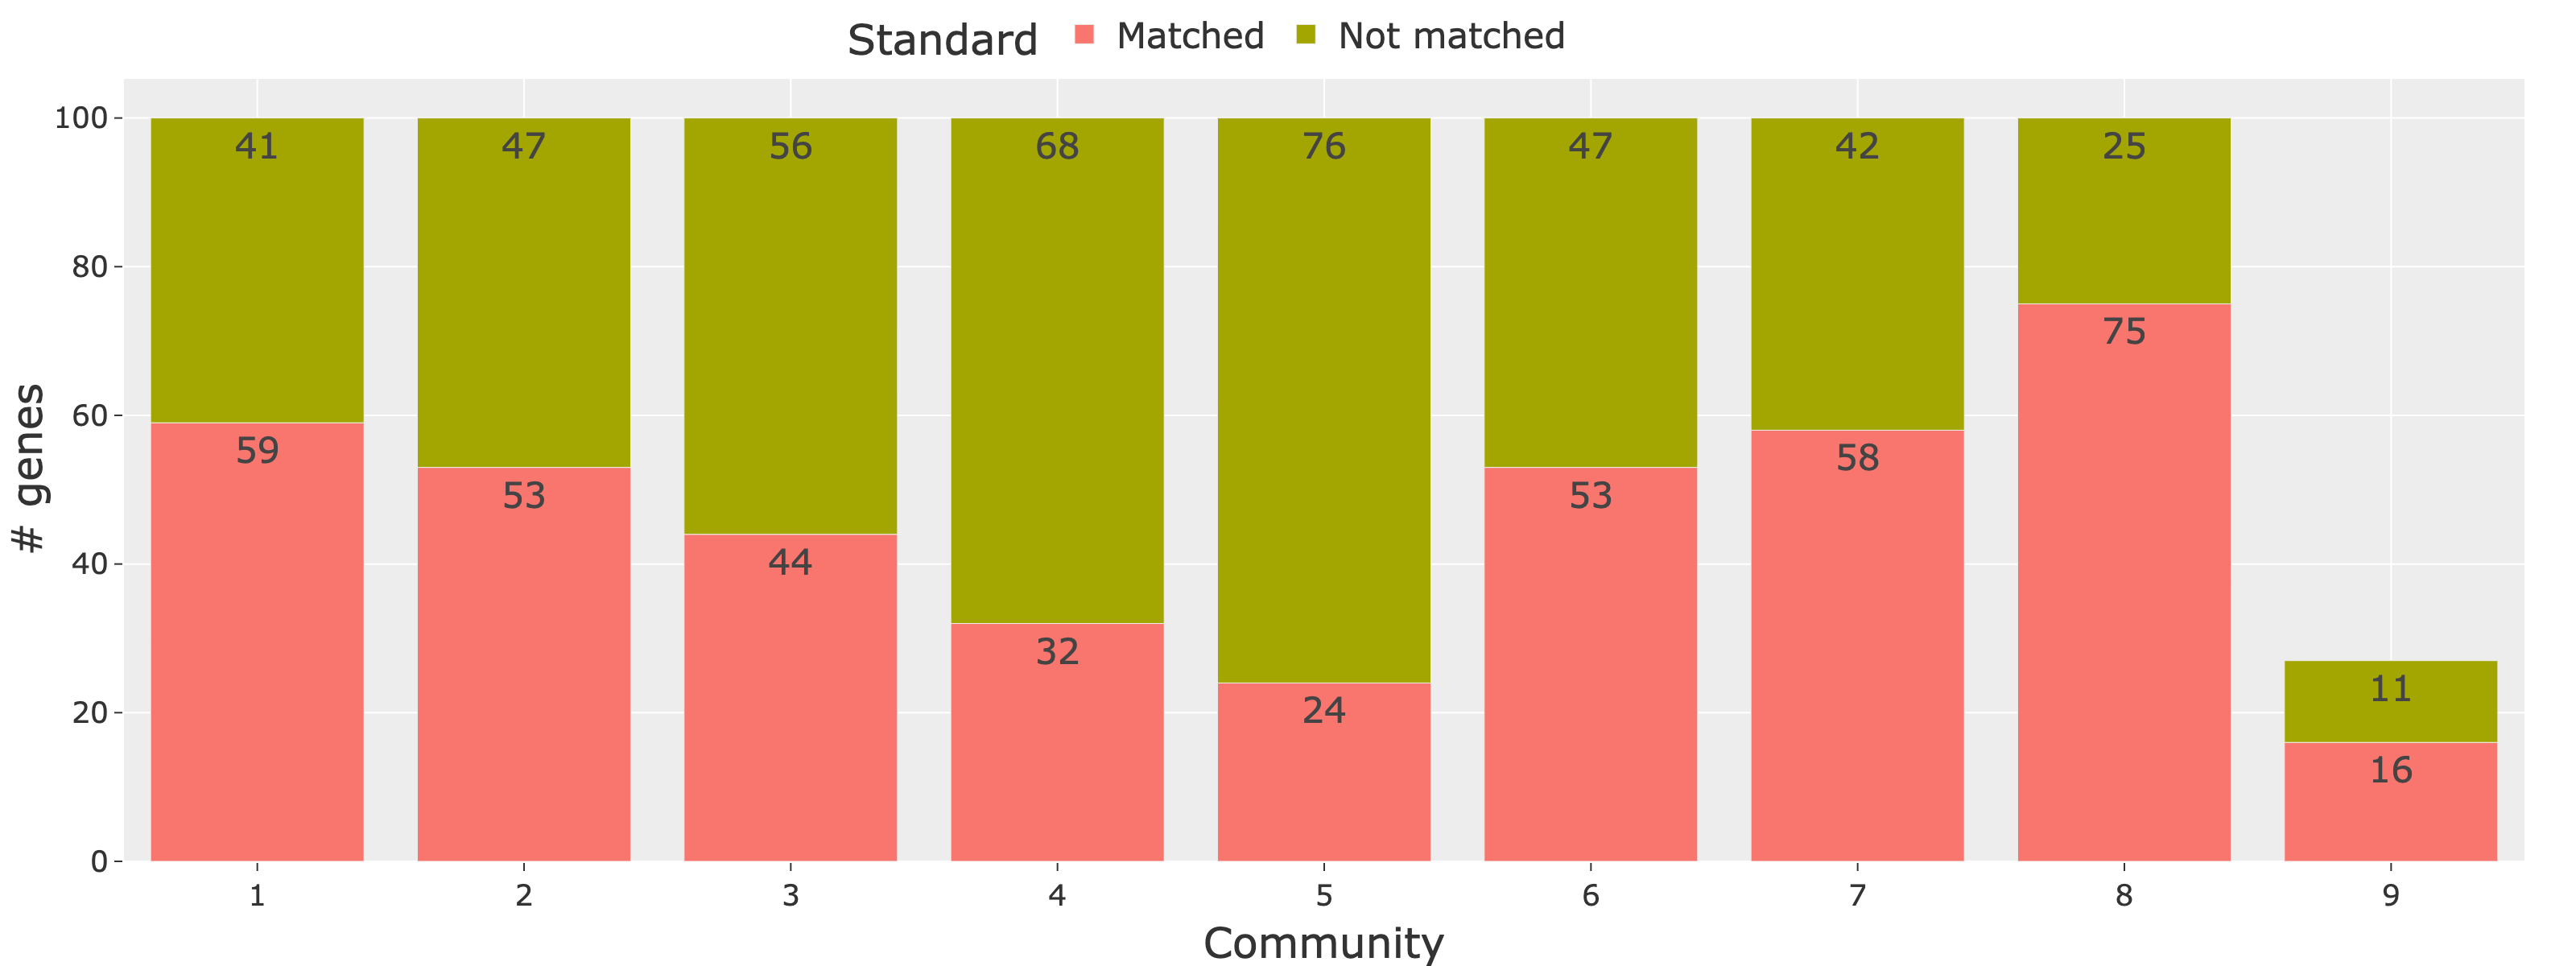
\includegraphics[width=\textwidth,keepaspectratio]{Sections/Network_I/Resources/P0/4K_p0_modConMev_rep_norm3_4K_50TF_v3.png}
        \caption{The most relative varied genes}
        \label{fig:N_I:p0_mev_sel_rep}
    \end{subfigure}
    \begin{subfigure}[b]{1.0\textwidth}
        \centering
        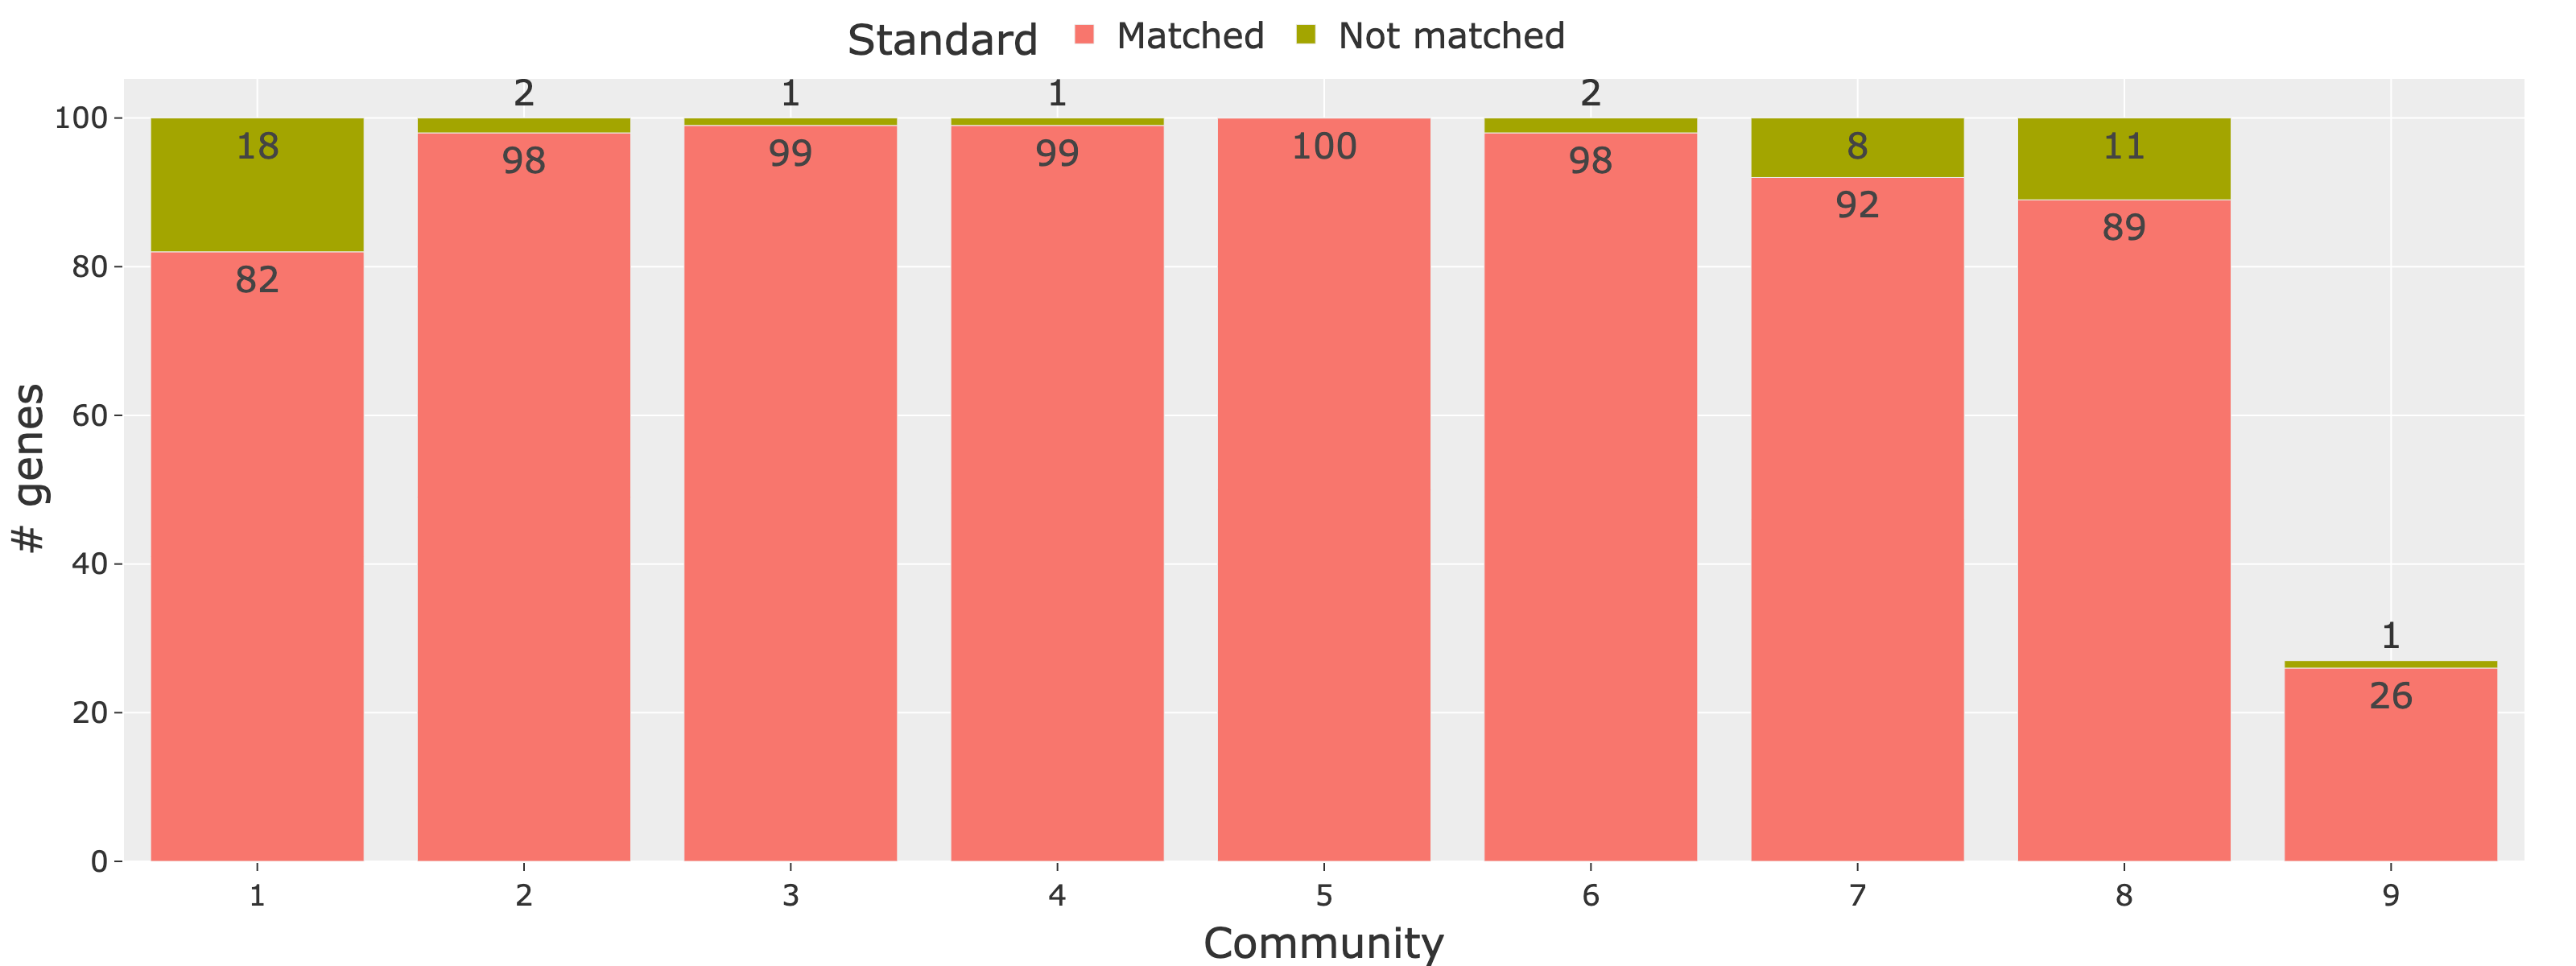
\includegraphics[width=\textwidth,keepaspectratio]{Sections/Network_I/Resources/P0/13K_p0_modConMev_rep_norm3_4K_50TF_v3.png}
        \caption{All the genes expressed}
        \label{fig:N_I:p0_mev_all_rep}
    \end{subfigure}
    \caption[Gene representation in MEV]{Genes found in the tumour dataset for the communities in the reward graph. The top 100 genes are selected by ModCon score. A) Is when the tumour dataset is restricted to the top most varied genes B) Includes all the expressed genes in the tumour dataset. The two plots show that using just the top 4000 most varied genes in tumour lead to a poor representation in the genes used to compute the MEVs.}
    \label{fig:N_I:p0_mev_rep}
\end{figure}



\subsection{Summary}

This section contains the first attempt in the project to integrate the non-healthy molecular information into MIBC subtyping by building a co-expressed network from the freshly isolated samples. The networks generated utilised the standard, reward, and penalised modifiers, with a minimum degree of 3 for standard genes and 50 for TF. The analysis performed in this section showed that the weight modifiers have an impact on both the network and the community detection algorithms but less so on the MIBC subgroups. 

% Limitation of using the top most varied genes
There are several limitations with the method presented in this section. The dataset consists only of P0 samples (only 23), so the network does not represent the other diverse tissue states as seen in the tumours. The gene expressions for both tumour and non-tumour datasets were aggressively filtered by keeping only the genes expressed in 90\% of the samples. There was also an additional filter of using just the 4000 most expressed genes in the tumours to compute the MEV which are the one used for MIBC stratification. These decision deepened the difference between the gene expression between the TCGA and the P0 samples which affected the MIBC subtypes derived from the three networks.

% Limitation of MEV
Another limitation of the MEVs was that the networks were used only as a gene selection mechanism, to extract the nodes which are highly connected inside a community. However, when it comes to computing the MEV only the expression from the tumour samples is used without taking in consideration the expression difference between the two datasets.

It was observed that choosing a larger minimum degree, 50 - P0 versus 6 - tumour derived networks, had a proportional effect on the networks metrics. The next chapter explores (\cref{s:N_I:sel_pruning}) in more detail the effects of selective edge pruning to the networks and the subgroups derived. 




% The next section studies the effects on the network pipeline, and implicitly on Leiden, when a subset of genes is prioritised at the edge pruning stage. In addition, the MEV only uses the gene expression for tumours, without fully integrating the two gene expression datasets. While this section did not generate useful biological findings, it was crucial in the development process.

% However, the experiments in this section and the work in \cref{s:ap:sel_prun} will show that allowing such a large number of TF has a big impact on the number of communities.


% % Reason 2 - Scatter biological pathways 
% Further on, when we look at the biology of each community we could see that there a lot shared pathways across communities. This include PDGF, CCKR, apoptosis and others. This gives the impression that the approach developed did the contrary from the intended behaviour, instead of isolating the biological processes it scattered through the network. The pathways were discovered through the Gene Ontology tool using PANTHER Pathway option and \textbf{no correction}; the latter because the majority of the genes inputted were \textbf{not} given significant results. This further strengthen our intuition that this approach is not providing the intended results.

% Figures I need to support for the above argument:
% \begin{itemize}
%     \item Pick 2-3 pathways from the ones found and highlight in the network.
%     \item Maybe put the Network with annotations?
% \end{itemize}

% % Reason 3 - Effect of the TF. but this really is 
% While performing the biological interpretation, looking at the genes selected by ModCon score, it can be clearly noticed that the TF genes play a major role in the networks. The reason for this is that in this set of experiment we enable 50 edges for each Transcription Factor, thus biasing the network for these genes. Definitely, this parameter have a large impact of ModCon. Therfore, we performed an experiment with a lower number of edges per TF and we found out that there are more communities with fewer communties.
% Figure supporting the above:
% \begin{itemize}
%     \item How many of the genes selected from the ModCon are a TF? Give some stats
%     \item The sub-graph where only the ModCon genes are selected for each community; with the size of the TF \ref{fig:N_1:tf_comp}
% \end{itemize}

